\section{Question 1}

\subsection{The Question}

\begin{flushleft}

We know the result of the Karate Club (Zachary, 1977) split.
Prove or disprove that the result of split could have been predicted
by the weighted graph of social interactions.  How well does the
mathematical model represent reality?

Generously document your answer with all supporting equations, code,
graphs, arguments, etc.

Useful sources include:

* Original paper

\url{http://aris.ss.uci.edu/~lin/76.pdf}

* Slides

\url{http://www-personal.umich.edu/~ladamic/courses/networks/si614w06/ppt/lecture18.ppt}

\url{http://clair.si.umich.edu/si767/papers/Week03/Community/CommunityDetection.pptx}

* Code and data

\url{http://networkx.github.io/documentation/latest/examples/graph/karate_club.html}

\url{http://nbviewer.ipython.org/url/courses.cit.cornell.edu/info6010/resources/11notes.ipynb}

\url{http://stackoverflow.com/questions/9471906/what-are-the-differences-between-community-detection-algorithms-in-igraph/9478989#9478989}

\url{http://stackoverflow.com/questions/5822265/are-there-implementations-of-algorithms-for-community-detection-in-graphs}

\url{http://konect.uni-koblenz.de/networks/ucidata-zachary}

\url{http://vlado.fmf.uni-lj.si/pub/networks/data/ucinet/ucidata.htm#zachary}

\end{flushleft}
\subsection{The Answer}

The intuitive approach to determining communities that arise from the original graphs is to successively remove edges of high importance until two disconnected clusters are produced. This idea is very broad are requires the definition of a few concepts. Edges is high importance have large flow and connect large areas of the graph. By removing these edges parts of the graph that are not clustered become disconnected as they were using these main edges to remain connected. The idealized scenario is that of two clusters connected by the edge of two bridge nodes. In this situation the edge is service the path spanning across the two clusters and will have large importance in the structure of the group. 

The idea of edge importance can be quantified with the definition of edge betweenness. Edge betweenness is the amount of ``flow'' and edge carries between all pairs of nodes where a signle unit of flow between two nodes divides itself evenly among all shortest paths between the nodes. The central idea of this definition is that flow can be represented by the number of shortest paths that span an edge. If an edge is used frequently in the shortest path between two nodes then it is important or central to the graph. Betweenness centrality is one measure of the centrality of a graph. 

The divisive approach to community detection is centered on this notion of removing nodes or edges that are central to the graph structure and observing the resulting graph for patterns. This is confirmed if we consider what the characteristics we expect in the factions contained in a graphs. Factions can be thought is as cliques were nodes are highly connected to each other and therefore have a high clustering coefficient. By removing the more prominent edges that are used by highly used to connect sections of the graph we remove the connections with low clusting and the result should make the groups of high connectivity more obvious. 

The Girvan-Newman algorithm is the quantification of these idea and can be summarized concisely in a few steps. 

\begin{itemize}
\item Compute the betweenenss of all existing edges in the network
\item Remove the edge with the highest betweenness
\item Repeat this process until the desired number of distinct clusters has formed. 
\end{itemize}

Following this algorithm leads to a result that is a fair apporximation of the actual division of the karate club. However, the result does contain some misclassifications. 


More accurate techiques exist that attemp to optimize a given quanity. One such method is the leading eigenvector method. This method optimizes the modality of the graph, which is a measure of the clustering or density of modules of the graph. The modularity matrix is defined:

\begin{center}


$ B_{vw} = A_{vw} - \frac{k_v k_w}{2m} $

\end{center}

By decomposing this matrix into eigenvectors the main components of modularity can be determined. The largest eigenvector is used to split the graph repeatedly in the direction of highest modality. Using this method resulted in an accurate prediction of the actual data of the karate club. 



\lstset{
    language=R,
    label=code:q1,
    caption={R code that performs that community detection}
}
\lstinputlisting{../karate.r}



\begin{figure}[H]
\centering 
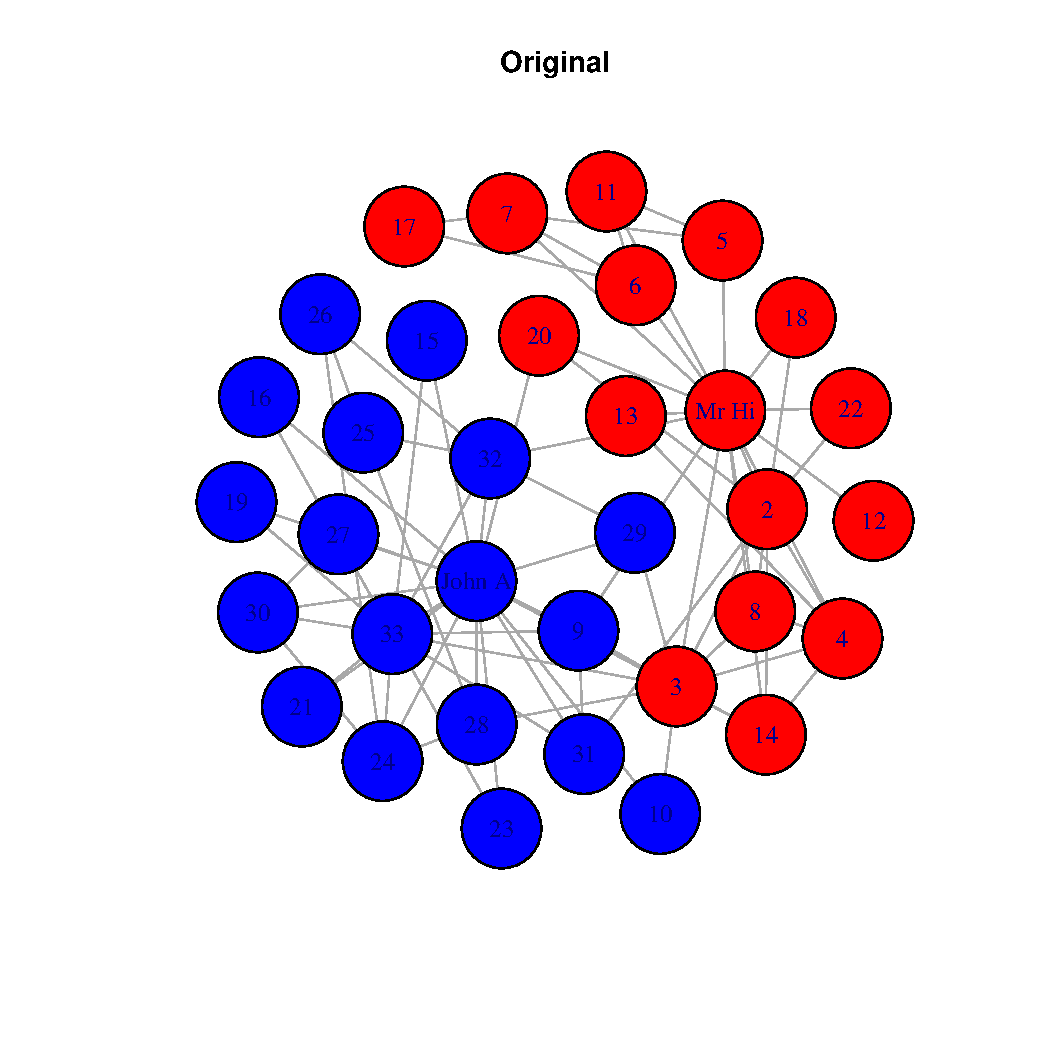
\includegraphics[width=.8\textwidth]{../Rplots.pdf}
\caption{Original partinioning based on data}
\end{figure}

\begin{figure}[H]
\centering 
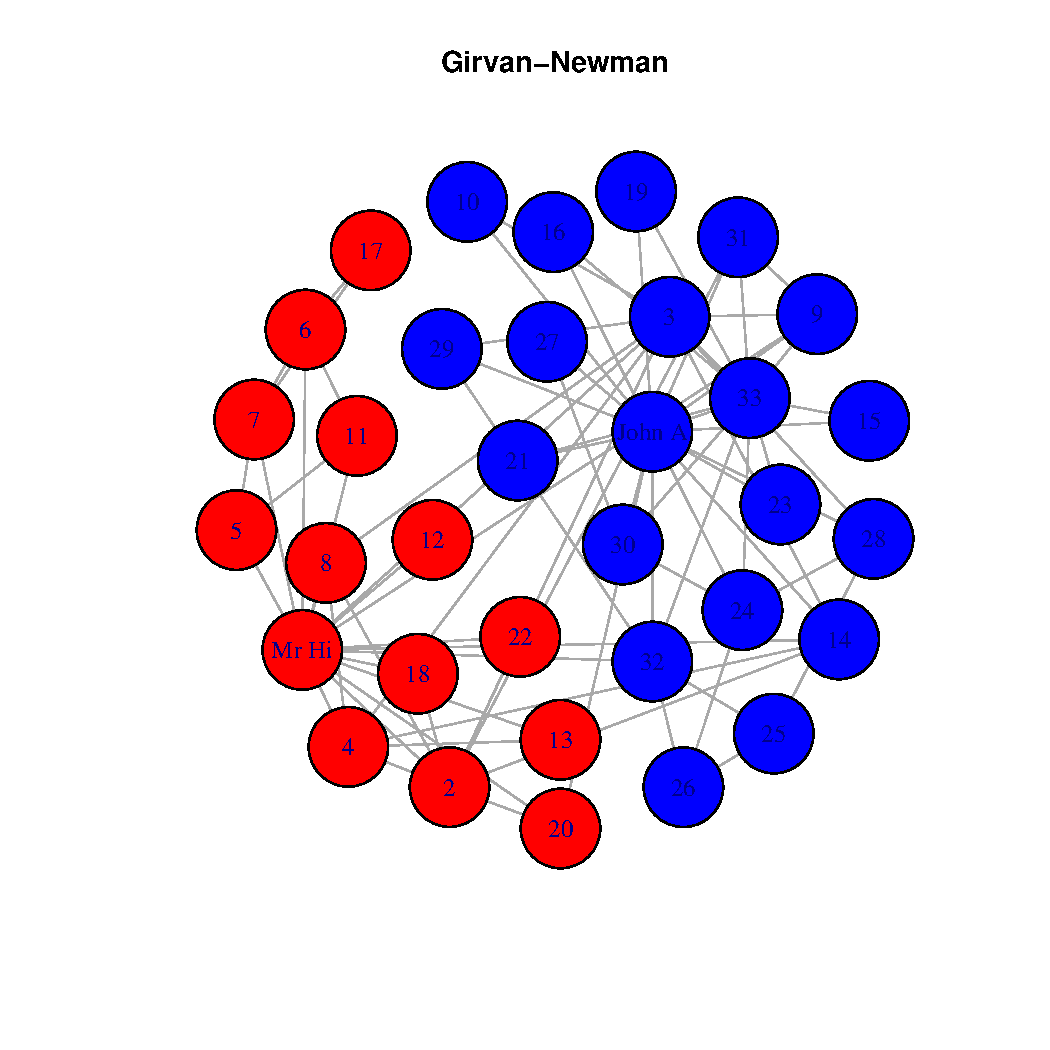
\includegraphics[width=.8\textwidth]{../Rplots1.pdf}
\caption{Predicted partitioning based on Girvan-Newman}
\end{figure}

\begin{figure}[H]
\centering 
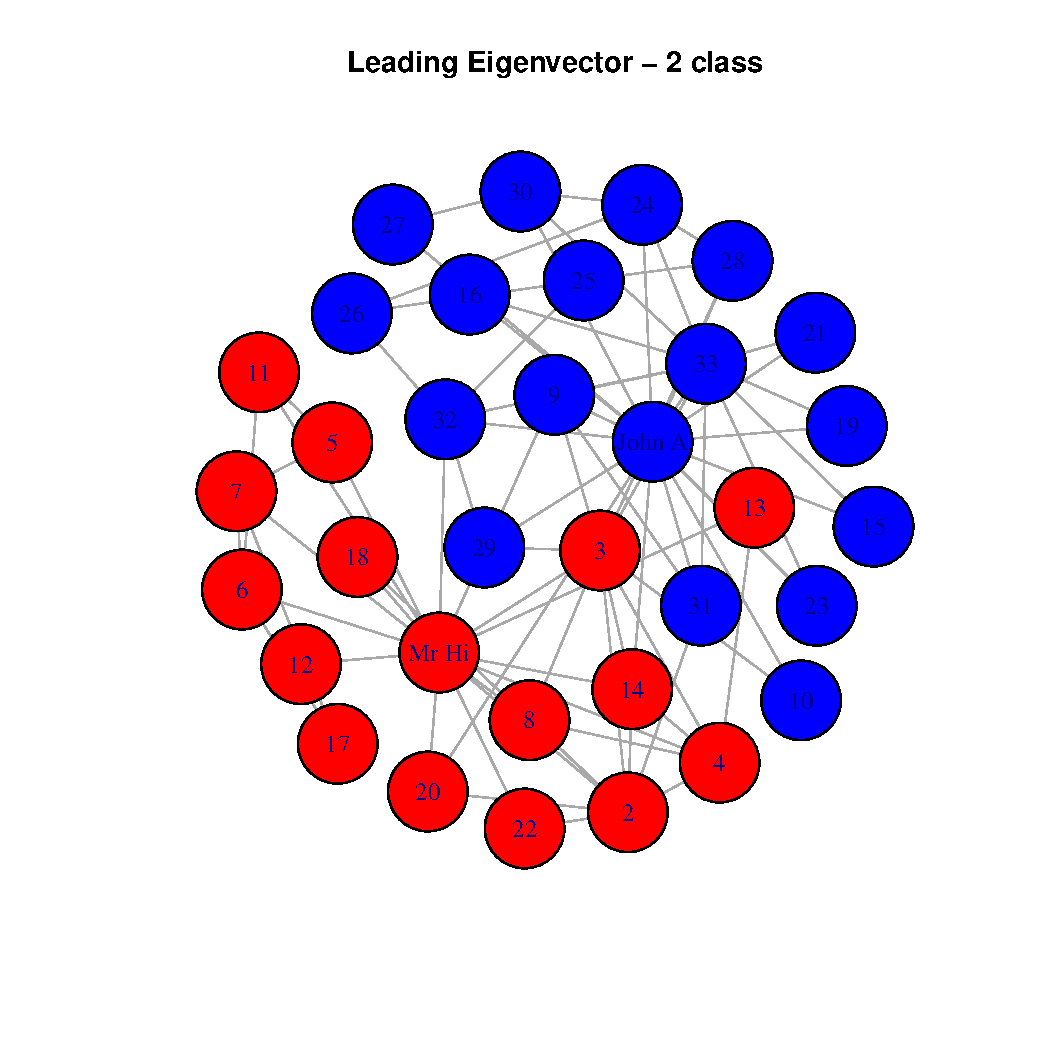
\includegraphics[width=.8\textwidth]{../Rplots2.pdf}
\caption{Predicted partitioning based on Leading Eigenvector Method}
\end{figure}


%
%\lstset{
%    language=R,
%    label=code:q1,
%    caption={R script to do the maths and plot}
%}
%\lstinputlisting{../q1/maths.r}
%%
%\lstset{
%    language=bash,
%    label=code:q1_test,
%    caption={Bash script to extract text from webpage, ignoring links}
%}
%\lstinputlisting{../process.sh}






